%%%% fs-run-barrier Barrier
\label {fs-barrier}

After processing, resulting items are collected in the barrier. There are valid as well as invalid ones. Its time to properly define meta-information that meets FlameStream timing model (section X) and intoduce invalidation relation that allows to distinguish valid and invalid ones.

\subsubsection{Meta information}
The meta-information of data item is represented as {\it global time} and the trace of {\it local times}.

\[Meta := (GlobalTime, Trace)\]

Global time is assigned to data item once when the item enters the system. It is represented as the concatenation of milliseconds since the epoch start and the identifier of front. Firstly, such design makes it possible to maintain global time strongly monotonic within single front. Secondly, it avoids assigning the same global time for distinct input elements. Global times can be compared lexicographically.

\[GlobalTime := (frontTs, frontId)\]

Local time is the concatenation of logical time of operation and the ordinal number of output item which we call {\it child id}. The logical time is represented as simple items counter within each operation. Therefore, child id is required, because some jobs can generate multiple items from one, e.g. flat map. The items with the same child id are called {\it brothers}. When the item leaves the operation, its trace of local times is appended by new corresponding local time. The traces of local times can be compared lexicographically.

\[Trace := [LocalTime]\]
\[LocalTime := (logicalTime, childId)\]

Notably, in spite of the fact that initially there are no items with the same global time, they can be generated by some operations. The trace of local times is used to distinguish two elements with the same global time. The main purpose of such approach is to provide information for items invalidation. The metas can be compared lexicographically: initially by global time and then by the trace of local times. 

It is important to mention that our concept of meta-information is similar to vector clocks
\cite{fidge1988timestamps, mattern88virtualtime}. However, unlike vector clocks, meta-information provides for the total order of data items due to the global time.

Figure~\ref{logical-graph-ops-figure} shows the topology of each operation and how it affects the trace of local times.

\begin{figure}[htbp]
  \centering
  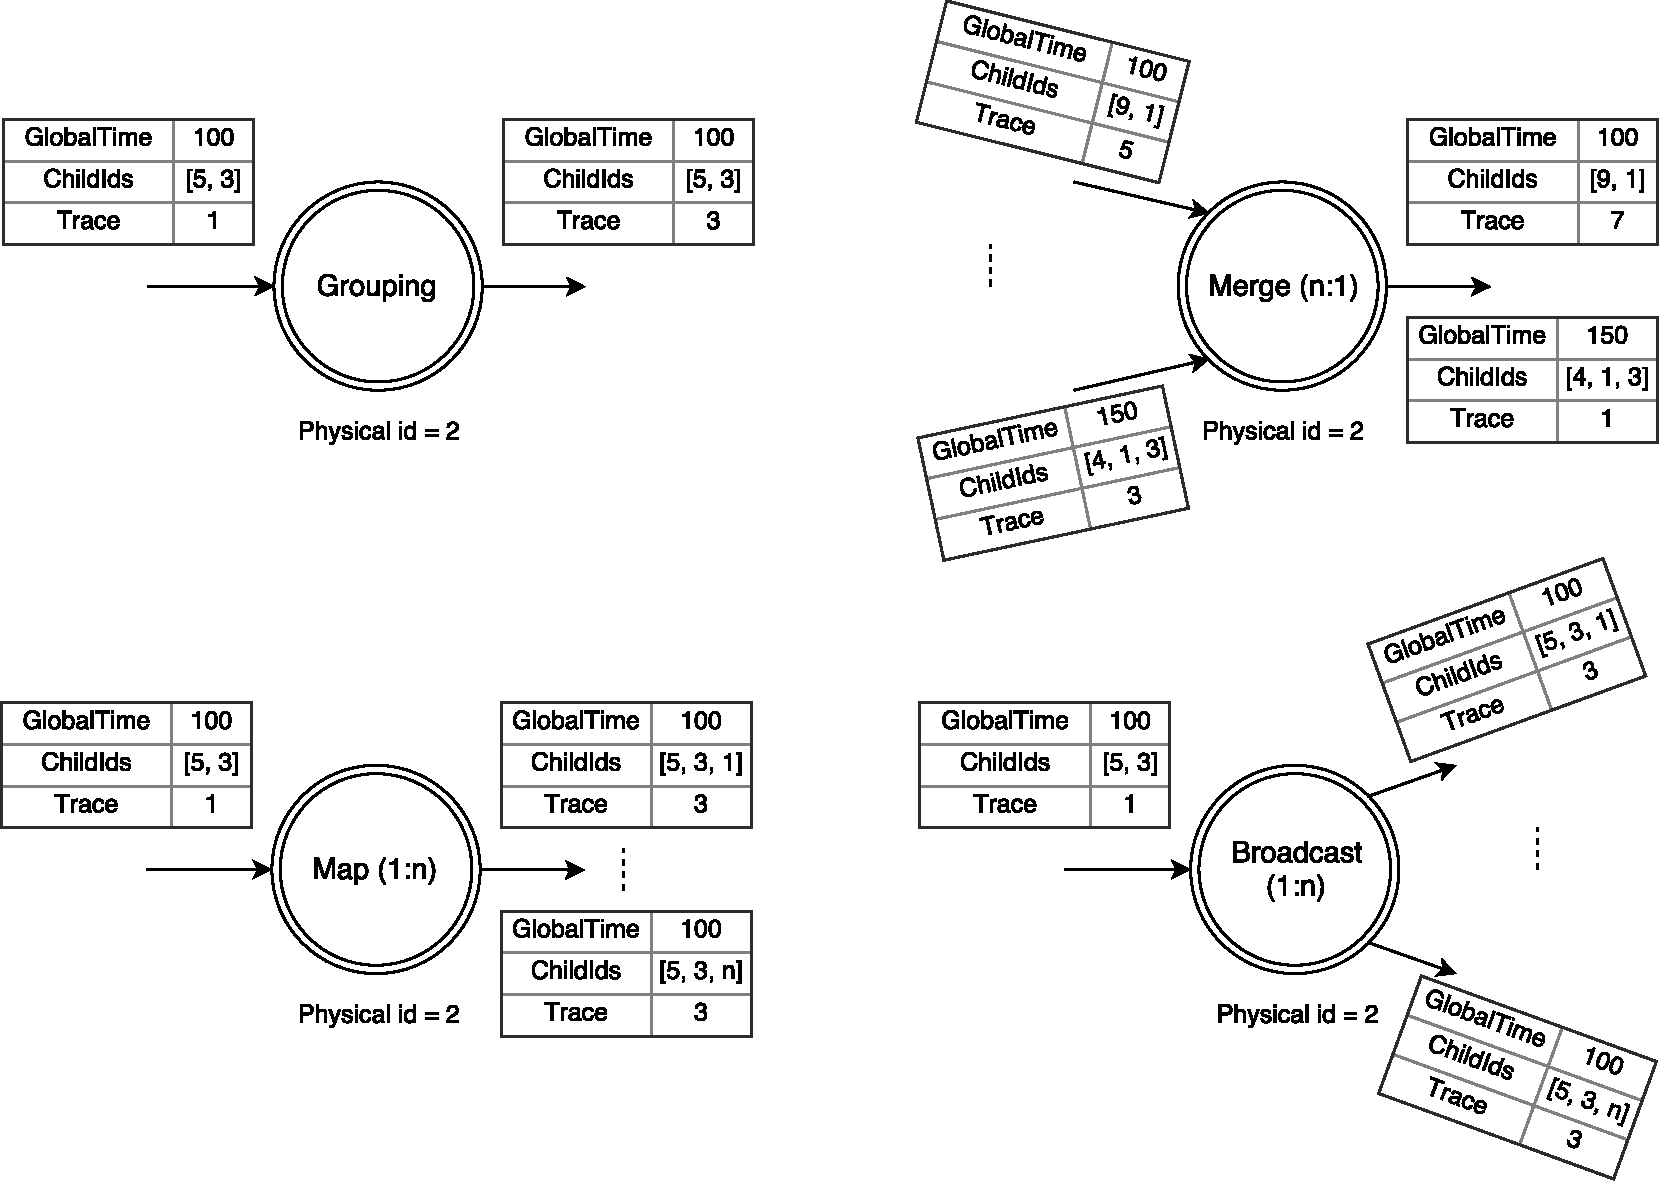
\includegraphics[scale=0.5]{pics/operations}
  \caption{Supported operations}
  \label {logical-graph-ops-figure}
\end{figure}

\subsection{Invalidation relation}

Replaying in grouping can generate incorrect tuples, multiple tuples with the same last item. Only one tuple from such set is correct. To find out which tuples are incorrect we introduce the invalidation relation between two data items. The main observation is that if there are two tuples with the same last elements, the one that the most recent on is more relevant that the previous one. 

The data item {\it A} is said to be invalidated by the data item {\it B} if:

\begin{enumerate}
\item They have the same global time
\item The trace of {\it A} is lexicographically less than the trace of {\it B}
\item The first difference is in logical time
\end{enumerate}

If the first difference is in child id, e.g. they were generated by broadcast operation, there is no invalidation relation between them. Hence, the invalidation relation is a partial order. 

Notice that the invalidation relation is defined not only on the grouping output, but on the all items. Stateless operation can not distinguish valid and invalid items and thy act on them as on the regular item. The invalidation relation cannot be lost, when item is go through other operations, because the trace of local times is append-only.

Barrier maintains a buffer for items. Once a new item arrives it inserts it in buffer and removes items that are invalidated by it.

However, there are two difficulties. Firstly, sinks are the parts of the physical graph, so they are also partitioned by the business-logic hash function. Hence, item and corresponding invalidation item can arrive to distinct barriers. Invalidating element has the same global time as the invalidee, so the partitioning of barriers by global time solves this problem. Secondly, it is unclear when the items should be released from the barrier. To do it the system should ensure that there are no in-flight items which can invalidate items in buffer. The solution of this problem is detailed in the next section. 

Figure~\ref{invalidation-problems-figure} illustrates possible sink issues. Red items with labels 4 and 7 got out from the system, despite the fact that they should be invalidated by corresponding green items. 

\begin{figure}[htbp]
  \centering
  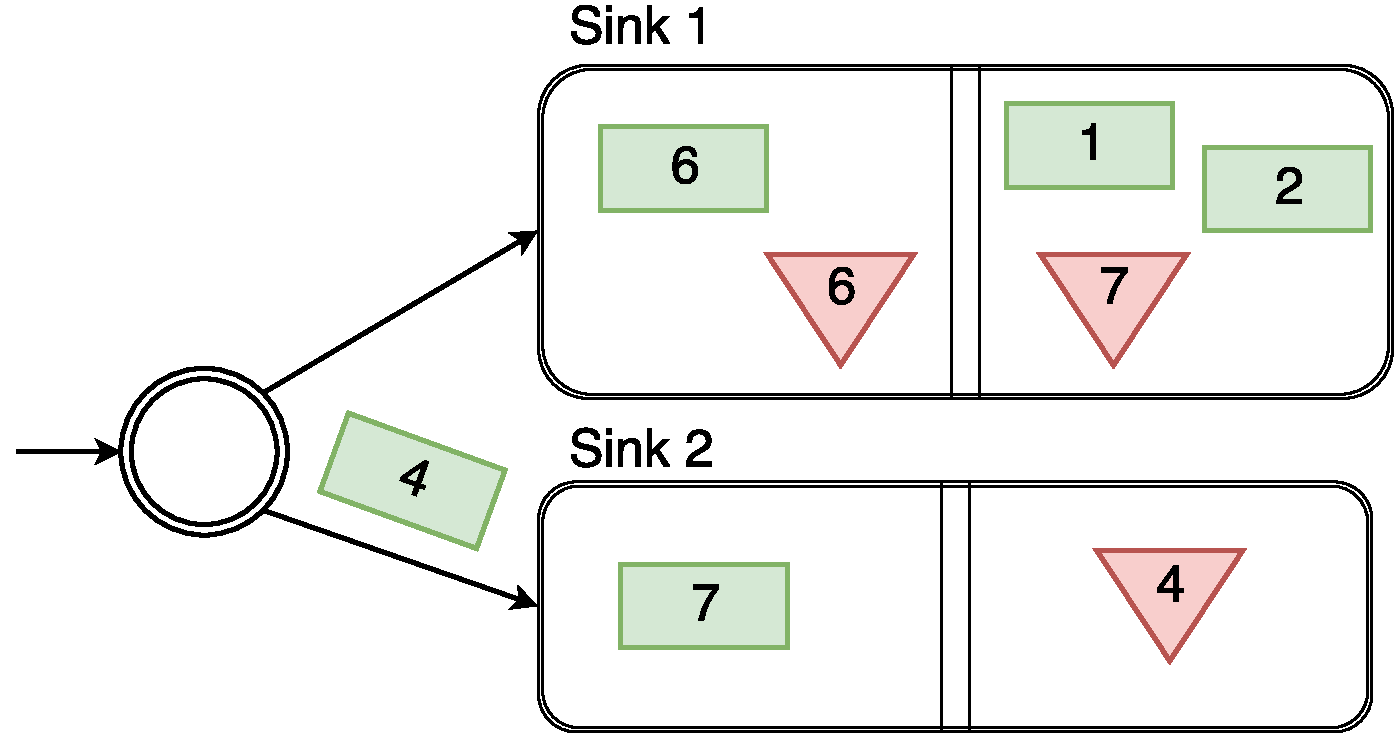
\includegraphics[width=0.48\textwidth]{pics/invalidation_problems}
  \caption{Possible sink issues}
  \label {invalidation-problems-figure}
\end{figure}
